\documentclass[]{article}
\usepackage{enumitem}
\usepackage{graphicx}

%opening
\title{Idea Marketplace | Seviss | Terence Brewer, Olivia Brewer, Steven Aque}
\author{Project 3: Storyboard Sketchup}

\begin{document}

\maketitle

\section{Background}
	Currently, there is nowhere on the Internet, at least indexed well, where someone can easily sell their personal intellectual property, including, but not limited to, ideas, consulting, fictional characters and premises, etc. so the desire for one to exist is what led to this project idea.
\section{Web Analysis}
	\begin{enumerate}
		\item Existing Sites That Are Relevant
		\begin{enumerate}
			\item Fiverr
			\begin{itemize}
				\item Posts organized in categories
				\item Reviews for posts
				\item Reviews as seller
				\item Direct communication with seller
				\item Website collects a portion of profits from seller
				\item Anyone can make an account and sell their service
				\item Customer is not producted from seller malicious practices
			\end{itemize}
			\item DeviantArt
			\begin{itemize}
				\item Search by popularity, new, and other filters
				\item Customizable user profiles
				\item Ability to follow users; display number of followers
				\item Promote postings through a group system
				\item Private and public messaging
				\item Comments on user profiles
				\item Pay for goods independently to seller
				\item Show related posts on listing
				\item Default dark theme
				\item Homepage features a gallery of images
				\item Images displayed in a grid-like fashion
				\item \(Shop\) user IP protected by copyrighted.com
				\item \(Shop\) premium currency can be used to make purchases
				\item \(Shop\) forced sign-in purchases
			\end{itemize}
			\item Amazon
			\begin{itemize}
				\item Pay to promote listings
				\item Recommendations for listings
				\item Save previous purchases
				\item Indirect communication with seller
				\item Protected purchase information
				\item left navbar contains a variety of search filters
				\item Product categorization through "departments"
				\item "Best sellers" list for product types
			\end{itemize}
			\item Ebay
			\begin{itemize}
				\item Option to auction goods
				\item Product categorization
				\item "Make an offer" option
				\item Any user can list products
			\end{itemize}
			\item AminoApps
			\begin{itemize}
				\item Store to purchase cosmetics such as stickers
				\item Recommendations on intial page
				\item Required login to post
				\item Divided into hundreds of communities
				\item Chatrooms
			\end{itemize}
			\item Craigslist
			\begin{itemize}
				\item Customer initiates sale through contact rather than "shopping cart" system
				\item Negotiable pricing
				\item Designed for users in close proximity
				\item Any user can list products
			\end{itemize}
		\end{enumerate}
		\item Functions We Want To Implement
		\begin{enumerate}
			\item Search products by name
			\item Filter search results
			\item Recommend products on login
			\item Pagination
			\item Copright-protect products
			\item Premium currency with ability to earn
			\item Ability to auction
			\item Security of user data
			\item Have an economy
			\item Create and customize a profile, including profile picture
			\item Private messaging with sellers and other users
			\item Forced login to post or purchase
			\item Products are reviewed before they are made public
			\item Chatrooms / public discussion
			\item Product categorization
			\item Seller Rating
		\end{enumerate}
		\item Table
		\begin{table}[!h]
			\begin{tabular}{|c|c|c|c|c|c|c|c|}
				\hline  & Our System & Fiverr & DeviantArt & Amazon & Ebay & AminoApps & Craigslist \\
				\hline Search & V & V & V & V & V & V & V\\
				\hline Filter & V & V & V & V & V & V & V\\
				\hline Recommend & V & V & V & V & V & V & X\\
				\hline Pagination & V & V & X & V & V & X & V\\
				\hline Copyright & V & X & O & X & X & X & X\\
				\hline Premium currency & V & X & V & O & O & V & X\\
				\hline Auction & V & X & X & X & V & X & O\\
				\hline Security & V & V & V & V & V & V & X\\
				\hline Economy & V & X & X & X & X & X & X\\
				\hline User Profile & V & X & V & X & X & V & O\\
				\hline Private message & V & V & V & O & O & V & X\\
				\hline Forced login & V & X & V & X & O & V & X\\
				\hline Reviewed by Site & V & X & X & V & V & O & X\\
				\hline Chatrooms & V & X & V & X & X & V & O\\
				\hline Categorization & V & V & V & V & V & V & V\\
				\hline Seller Rating & V & V & X & V & V & X & X\\ 
				\hline
			\end{tabular}
			\caption{V: Able to perform the task; X: Unable to perform the task; O: Able to perform the task with poor interactive design}
		\end{table}
	\end{enumerate}
\section{Storyboard}
	\begin{enumerate}
		\item Who is this site for? 
		Buyers and Sellers of Intellectual Property
		\item Storyboard Sketchup:
		\begin{itemize}
			\item Seller Perspective: Creating a product with existing account
		\end{itemize}
			\begin{figure}
			  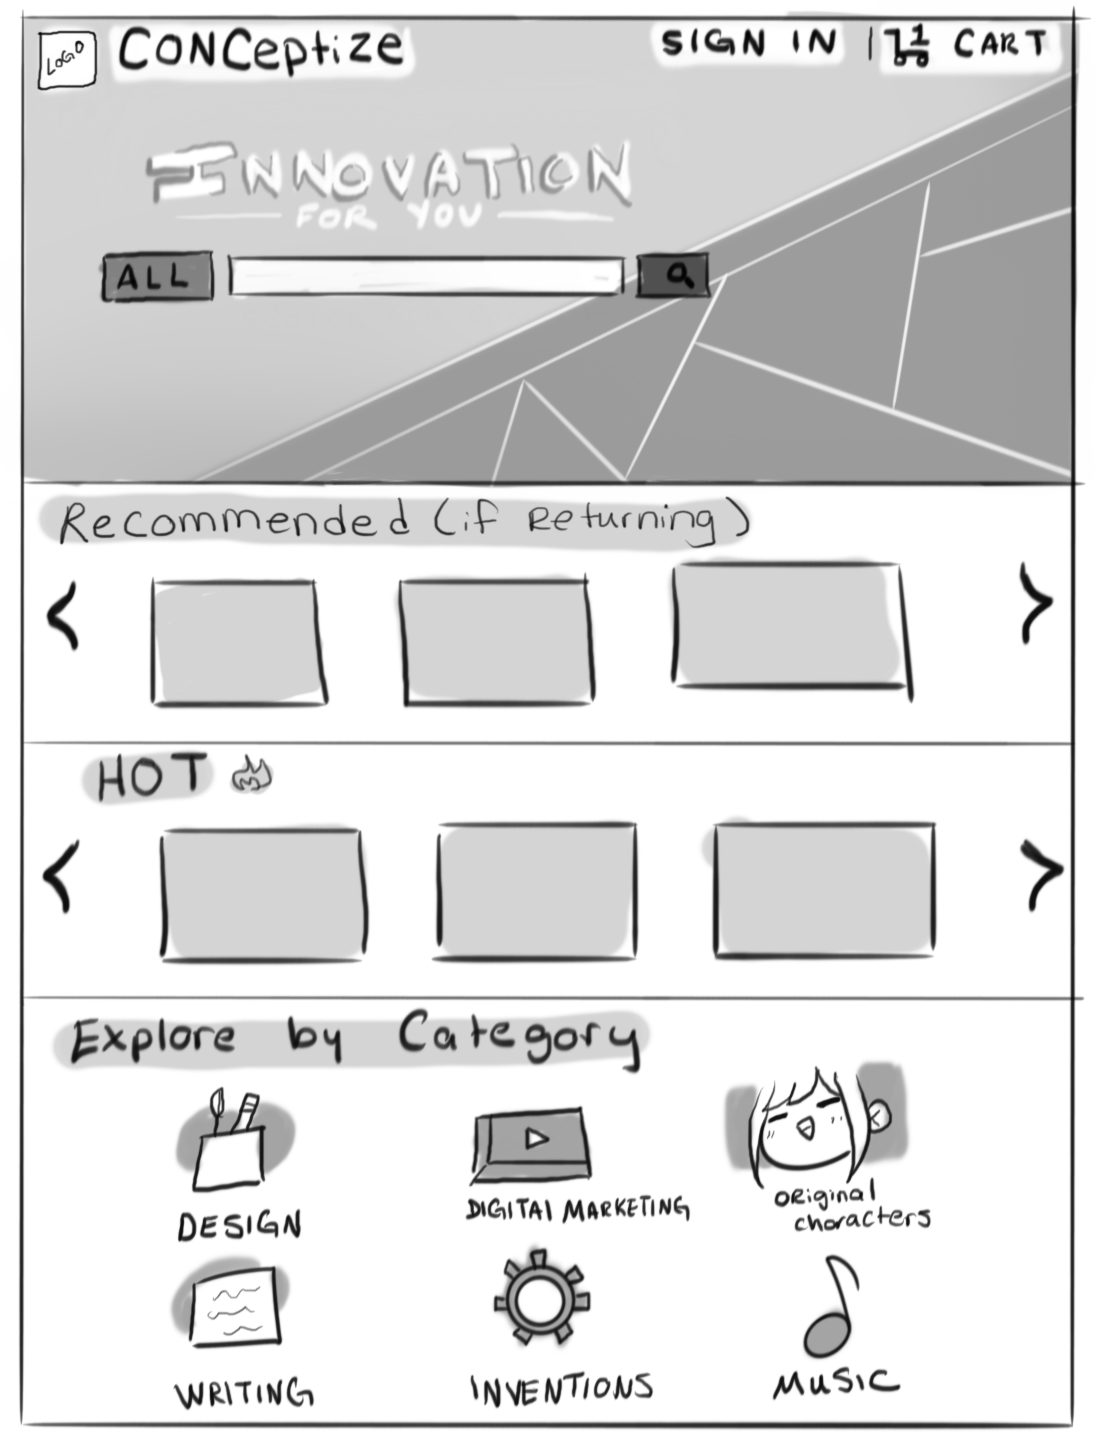
\includegraphics[width=\linewidth]{./pictures/homepage.png}
			  \caption{Arrive at homepage. Click sign in.}
			  \label{fig:seller1}
			\end{figure}
			
			\begin{figure}
			  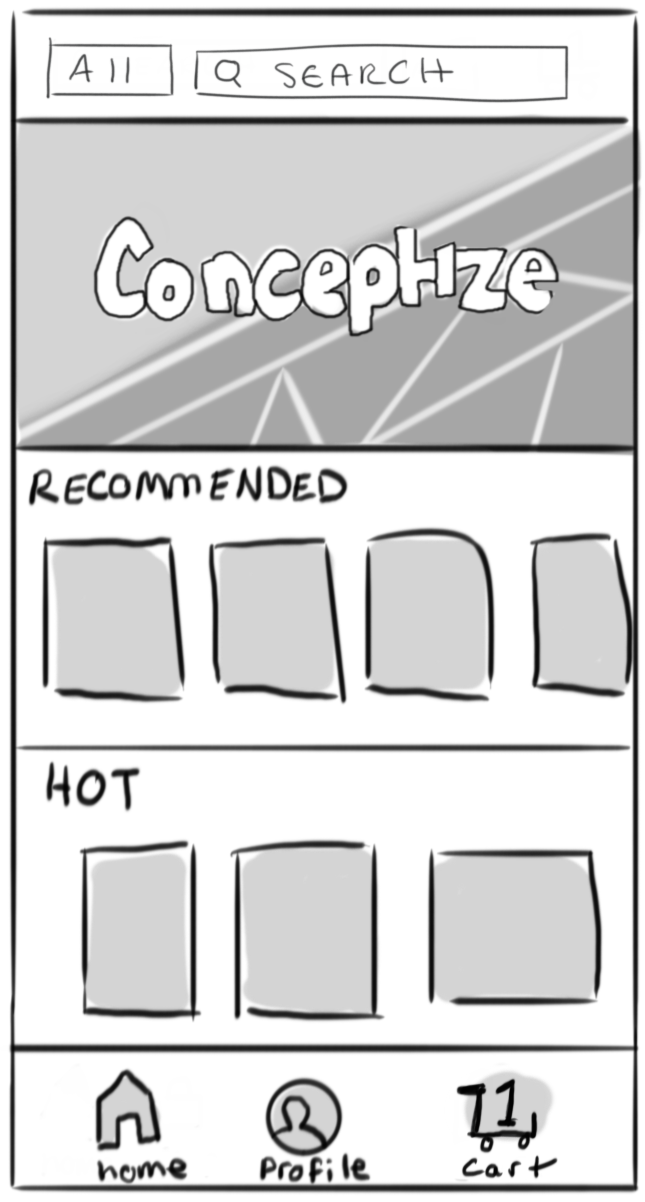
\includegraphics[width=\linewidth]{./pictures/homepage_mobile.png}
			  \caption{Mobile version.}
			  \label{fig:mobile1}
			\end{figure}			
			
			\begin{figure}
			  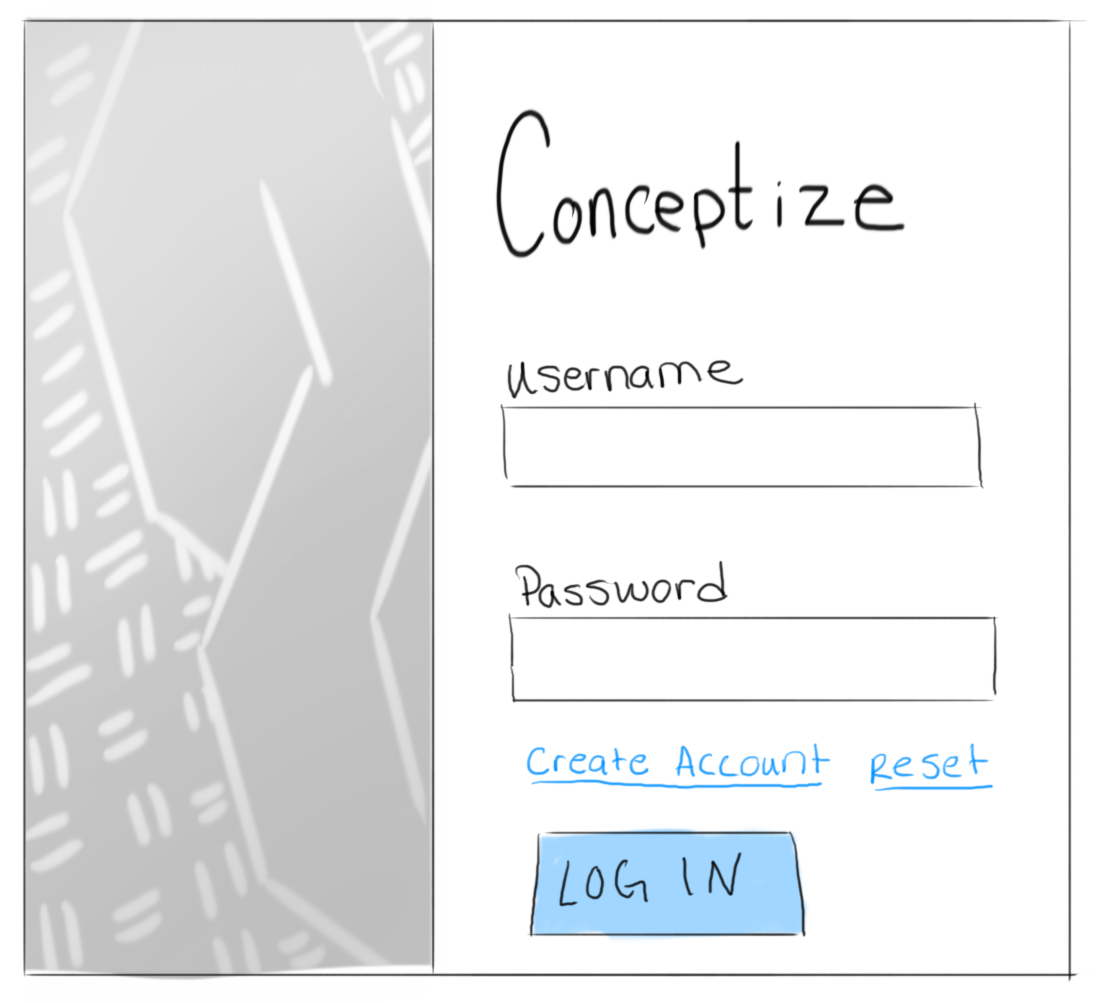
\includegraphics[width=\linewidth]{./pictures/login.png}
			  \caption{Sign in with valid credentials. Login proceeds to homepage (already listed). Click on profile to arrive at profile page.}
			  \label{fig:seller2}
			\end{figure}
			
			\begin{figure}
			  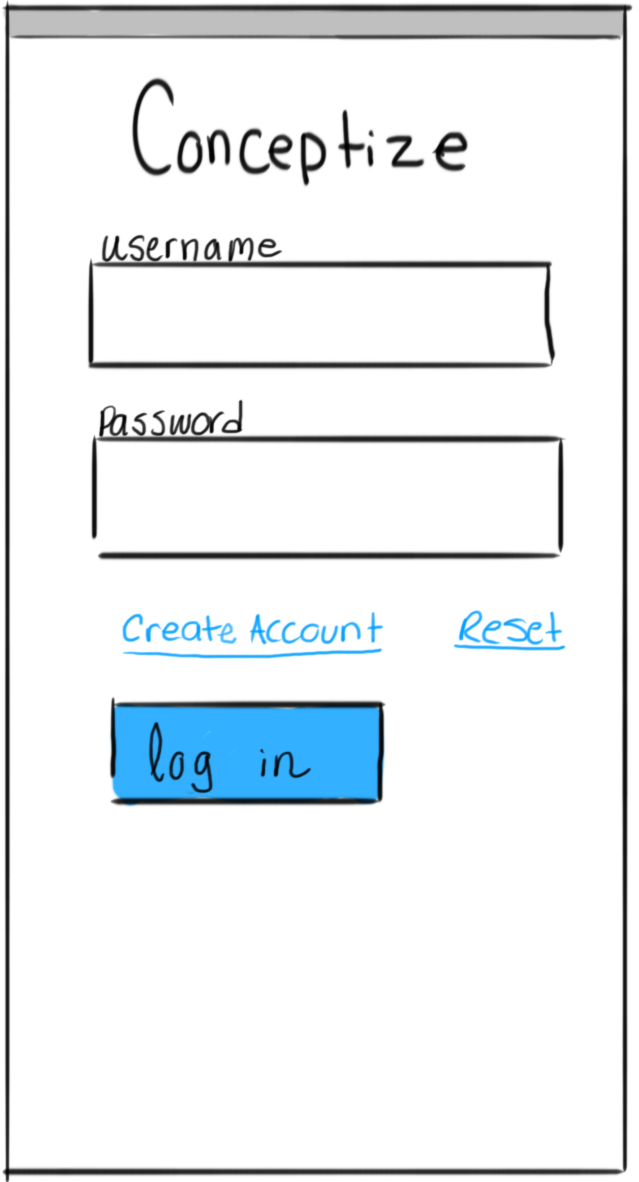
\includegraphics[width=\linewidth]{./pictures/login_mobile.png}
			  \caption{Mobile version.}
			  \label{fig:mobile2}
			\end{figure}
			
			\begin{figure}
			  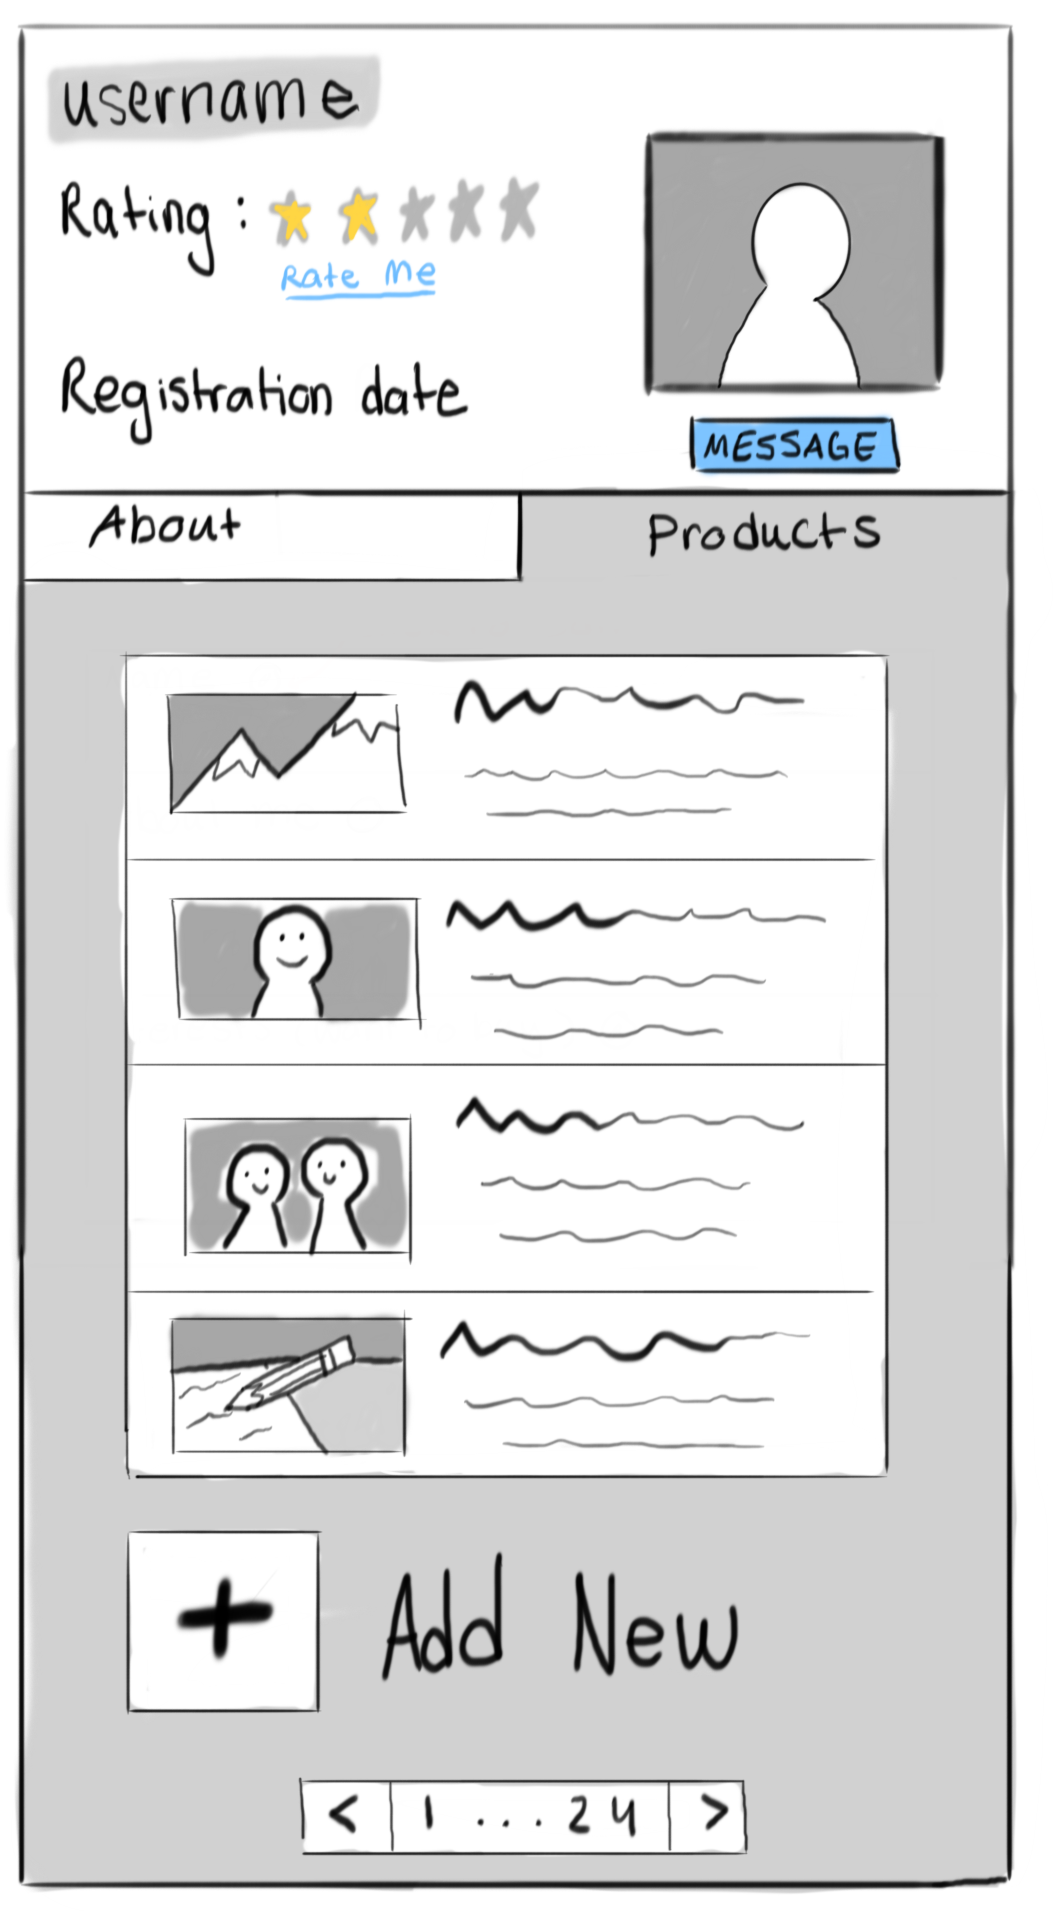
\includegraphics[width=\linewidth]{./pictures/profile_product.png}
			  \caption{User can edit profile, including adding a product with Add New}
			  \label{fig:seller3}
			\end{figure}
			
			\begin{figure}
			  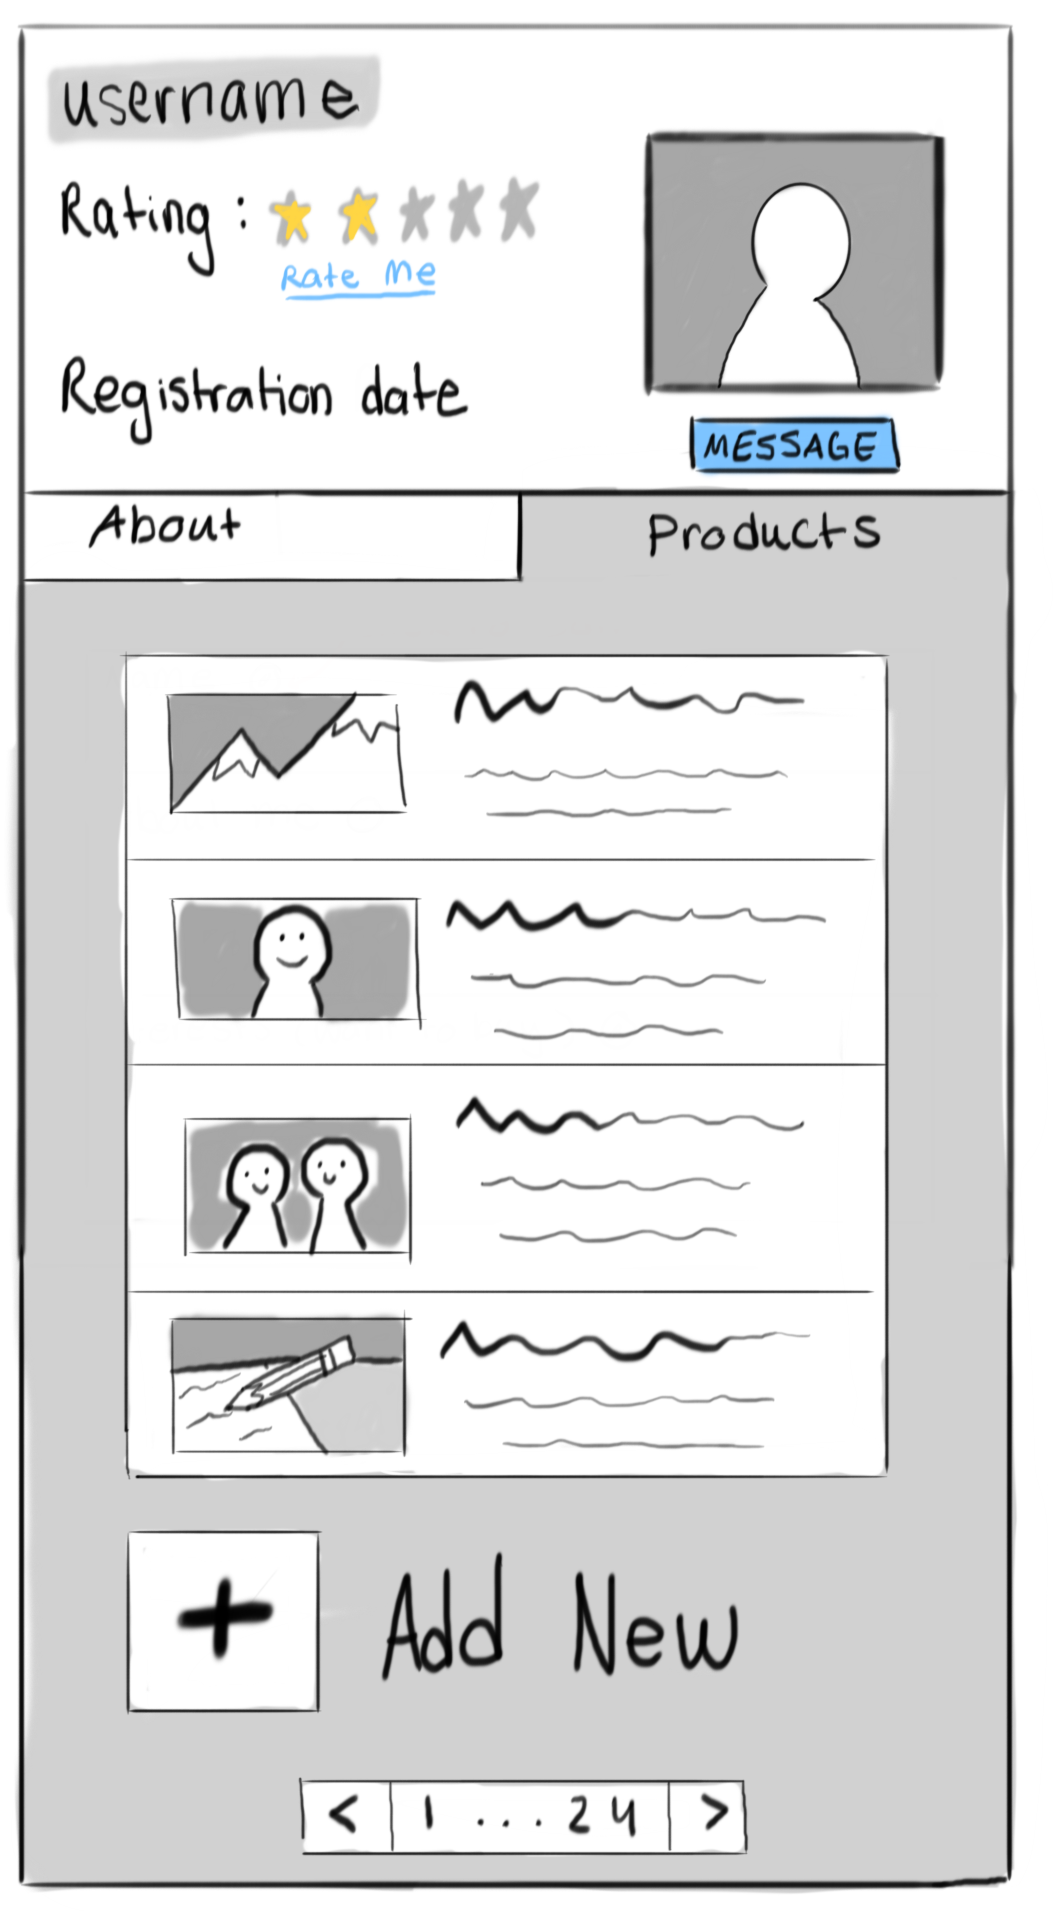
\includegraphics[width=\linewidth]{./pictures/profile_product.png}
			  \caption{Mobile version.}
			  \label{fig:mobile3}
			\end{figure}
			
			\begin{figure}
			  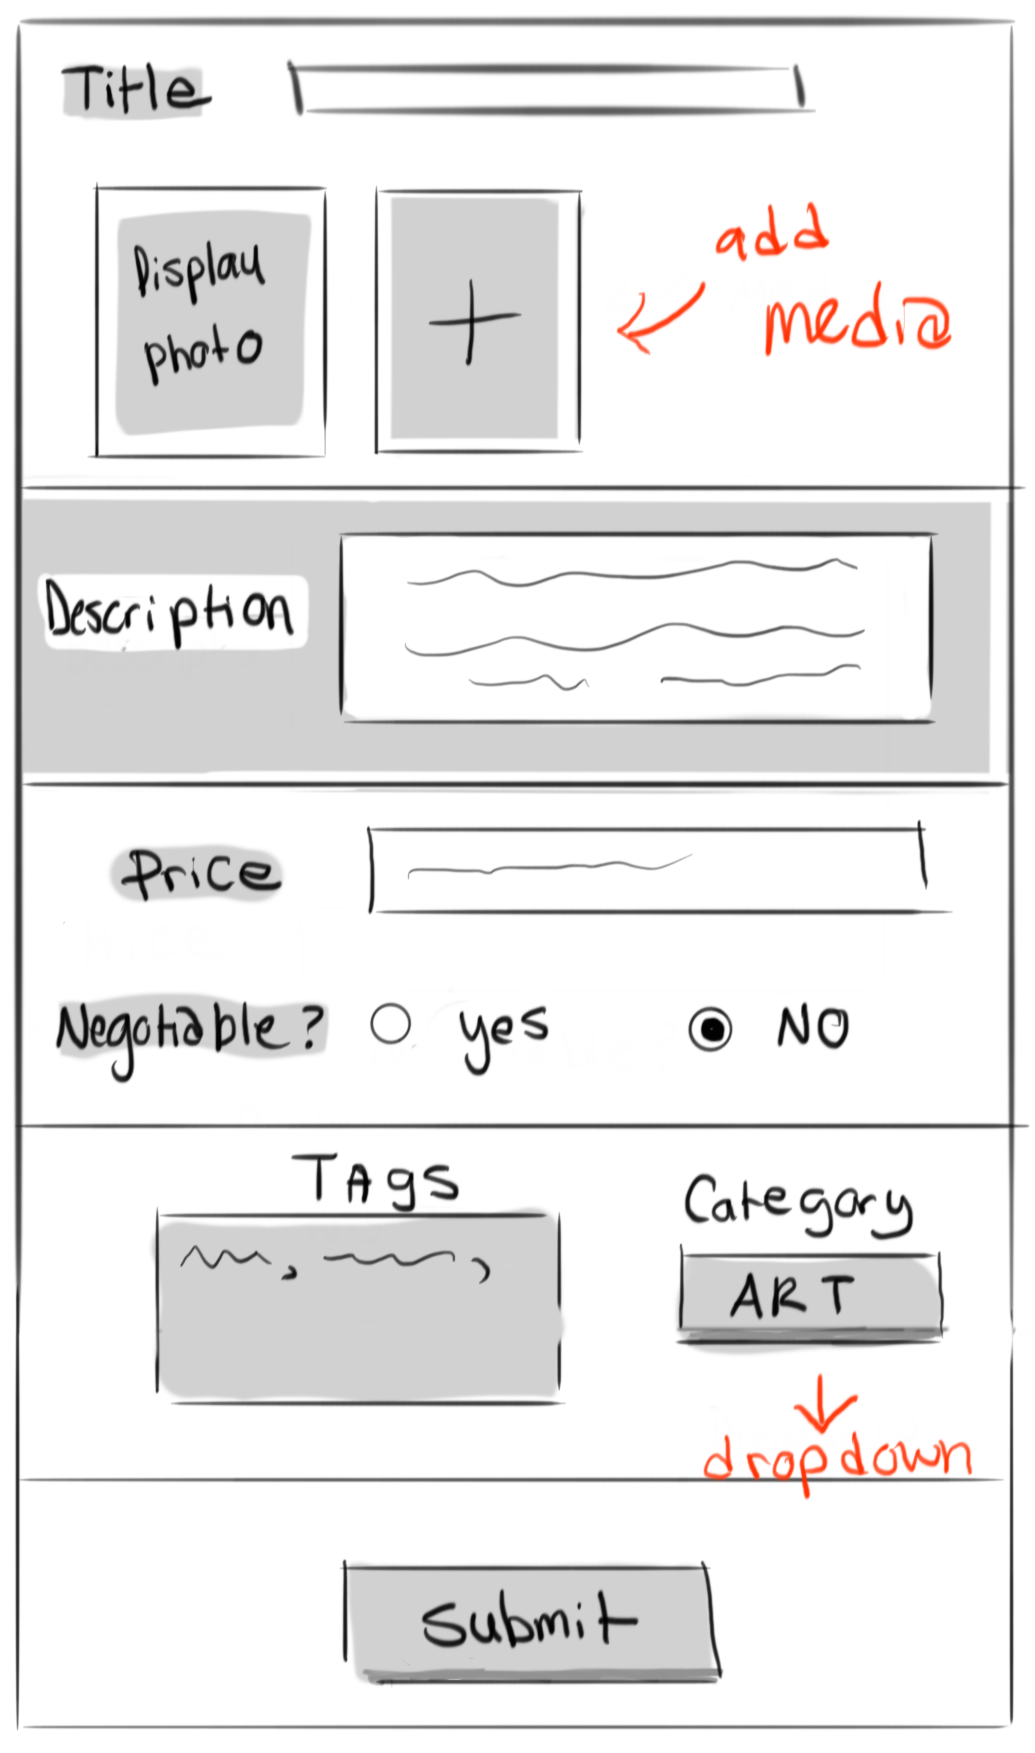
\includegraphics[width=\linewidth]{./pictures/create_page.png}
			  \caption{User can edit fields related to the product. User can then submit it.}
			  \label{fig:seller4}
			\end{figure}
			
			\begin{figure}
			  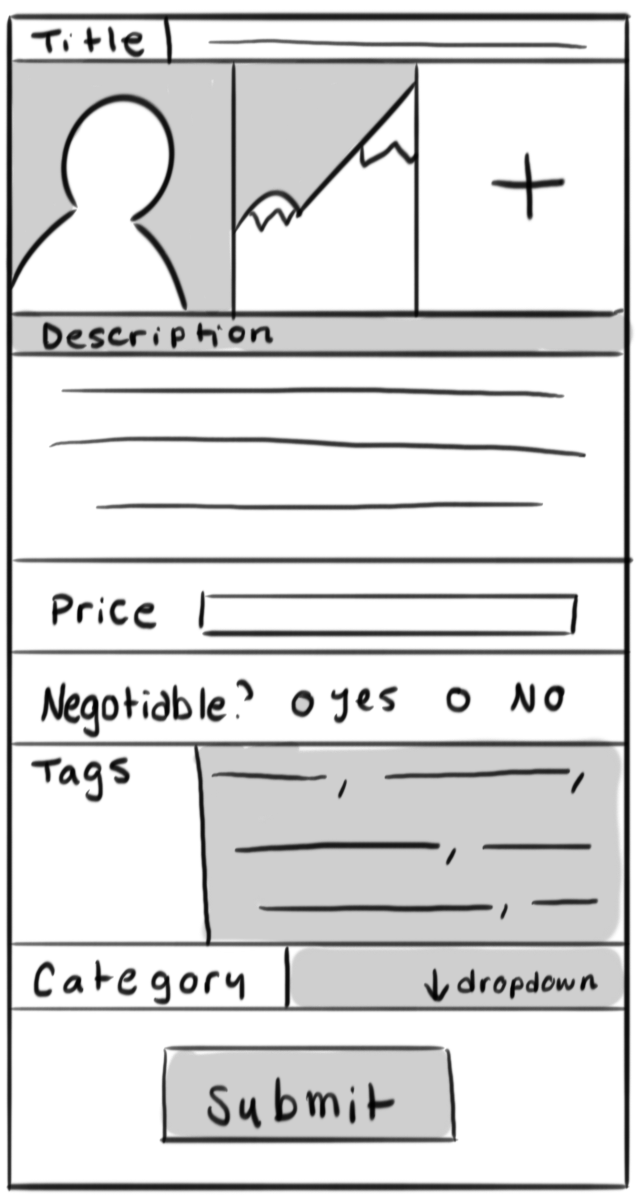
\includegraphics[width=\linewidth]{./pictures/create_page_mobile.png}
			  \caption{Mobile version.}
			  \label{fig:mobile4}
			\end{figure}
			
			\begin{figure}
				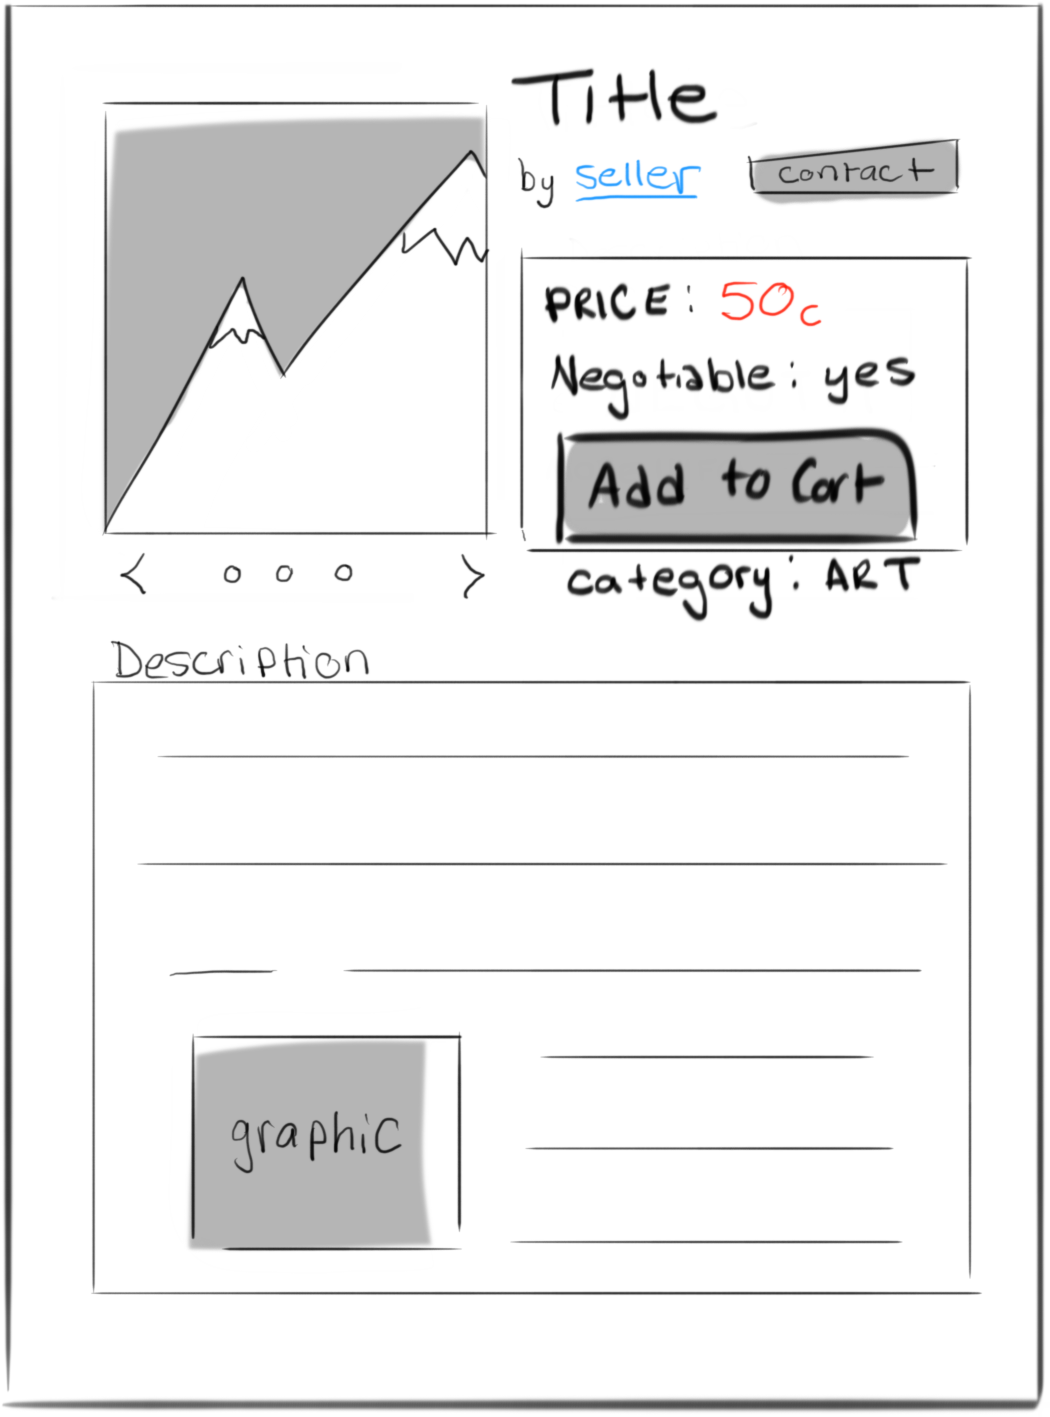
\includegraphics[width=\linewidth]{./pictures/product.png}
				\caption{The user can now see their product page live for everyone to see!}
				\label{fig:seller5}
			\end{figure}
			
			\begin{figure}
			  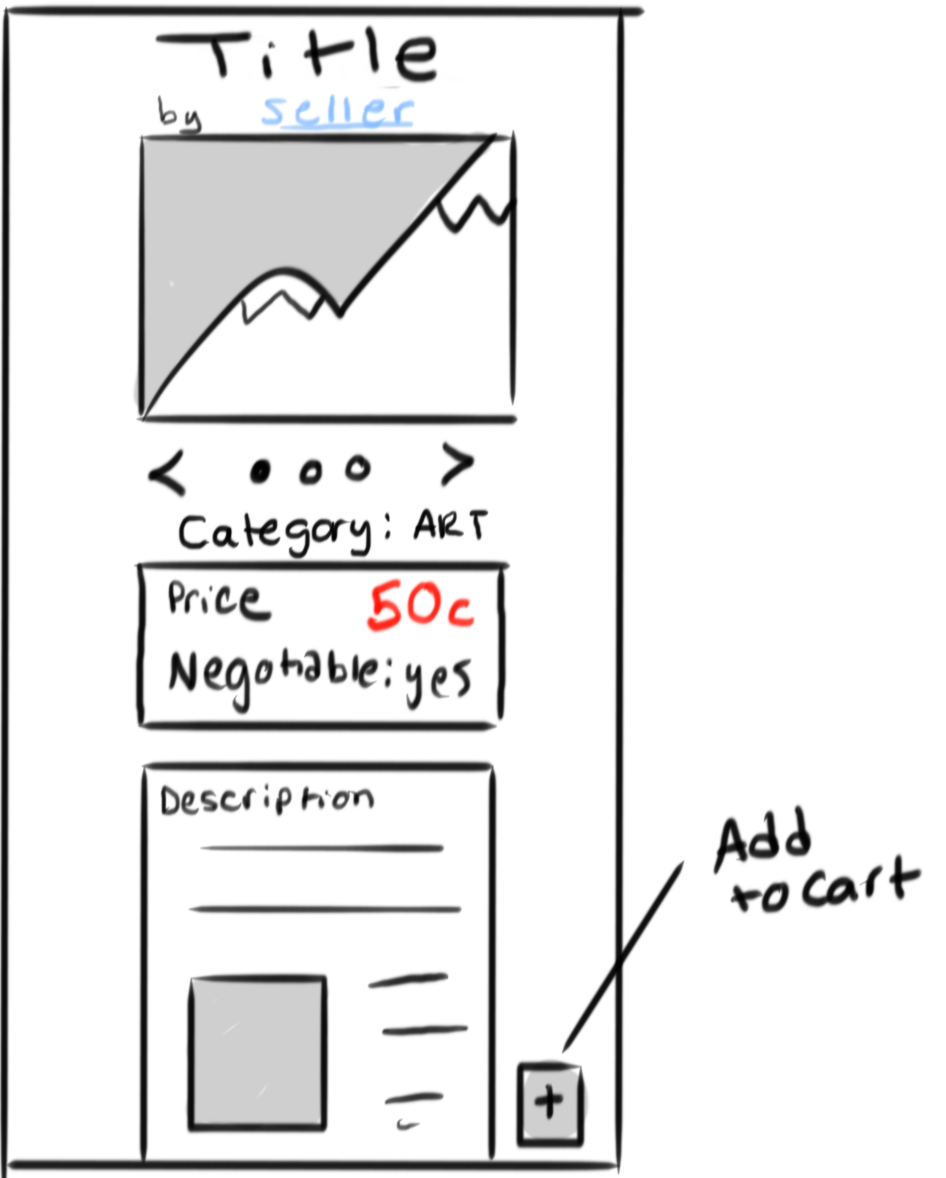
\includegraphics[width=\linewidth]{./pictures/product_mobile.png}
			  \caption{Mobile version.}
			  \label{fig:mobile5}
			\end{figure}
		\begin{itemize}
			\item Buyer Perspective: Buying a product using search without existing account
		\end{itemize}
		\begin{figure}
		  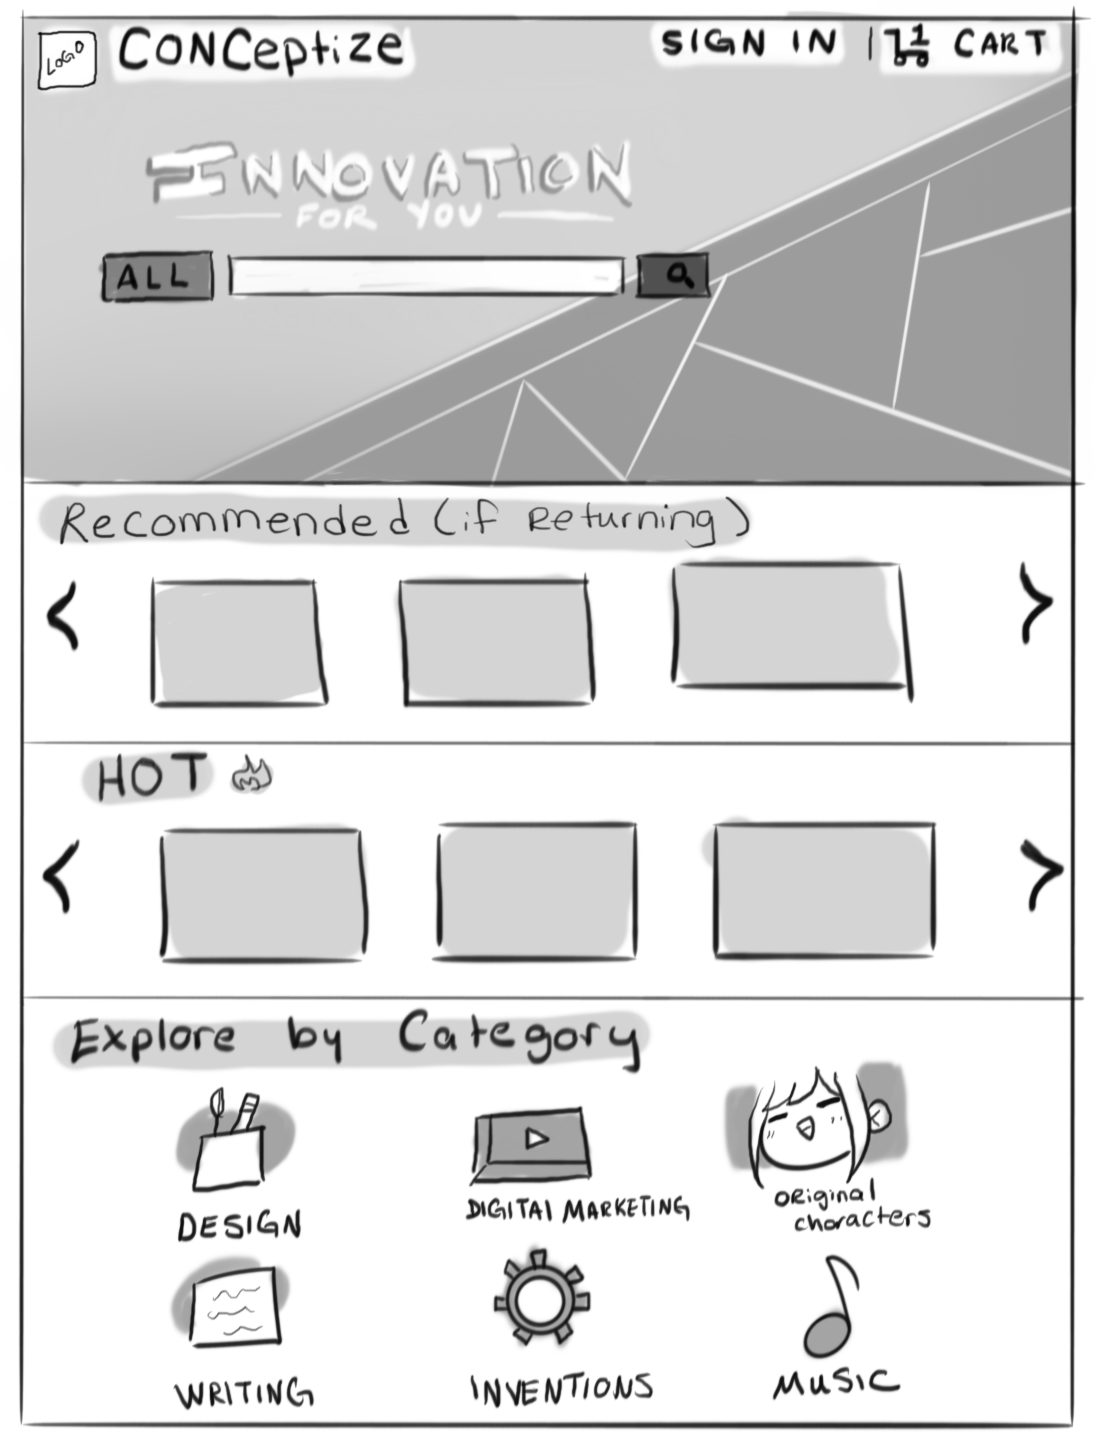
\includegraphics[width=\linewidth]{./pictures/homepage.png}
		  \caption{User arrives at homepage. Searches for product using search bar.}
		  \label{fig:buyer1}
		\end{figure}
		
		\begin{figure}
		  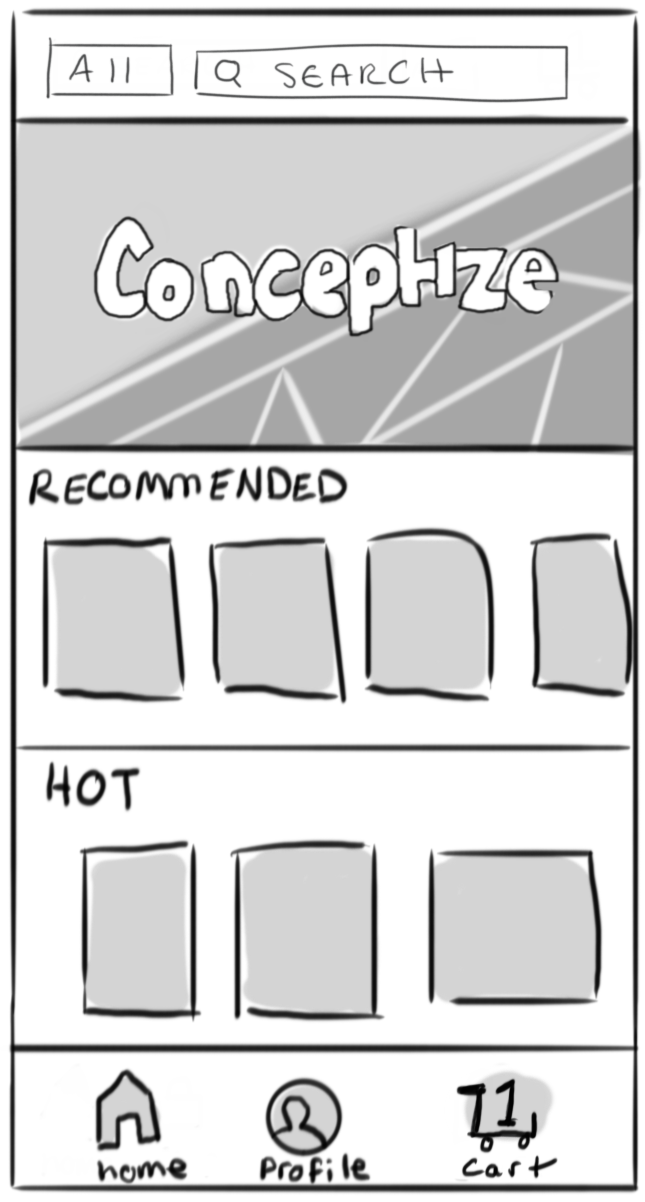
\includegraphics[width=\linewidth]{./pictures/homepage_mobile.png}
		  \caption{Mobile version.}
		  \label{fig:mobile6}
		\end{figure}
		
		\begin{figure}
		  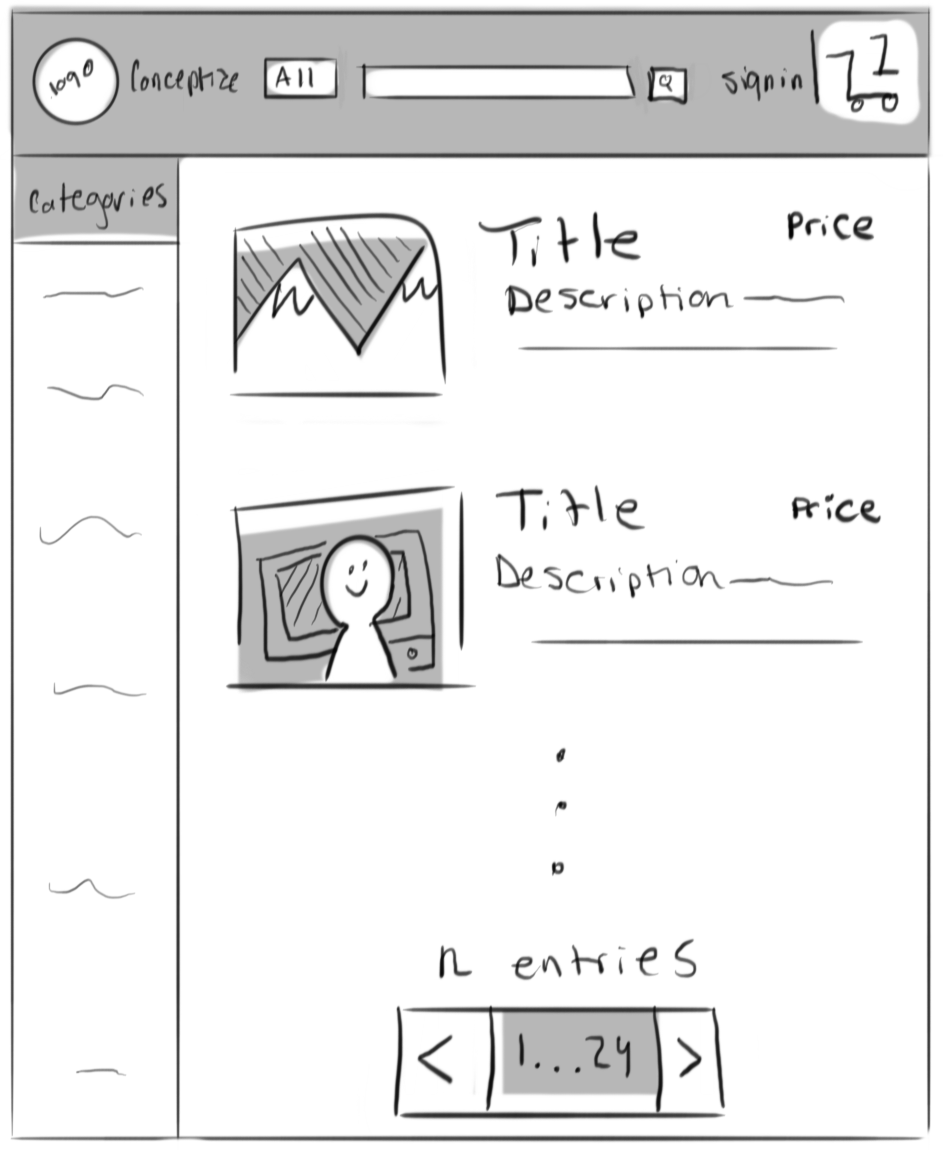
\includegraphics[width=\linewidth]{./pictures/search_results.png}
		  \caption{From the search results, the user chooses a product.}
		  \label{fig:buyer2}
		\end{figure}		
		
		\begin{figure}
		  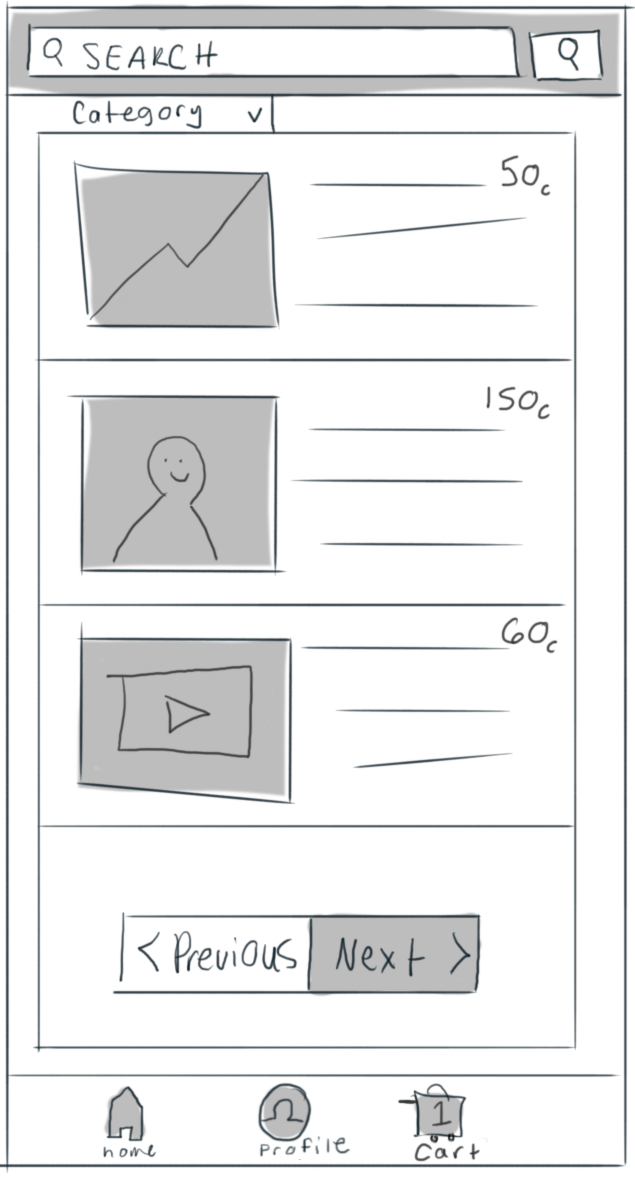
\includegraphics[width=\linewidth]{./pictures/search_results_mobile.png}
		  \caption{Mobile version.}
		  \label{fig:mobile7}
		\end{figure}
		
		\begin{figure}
		  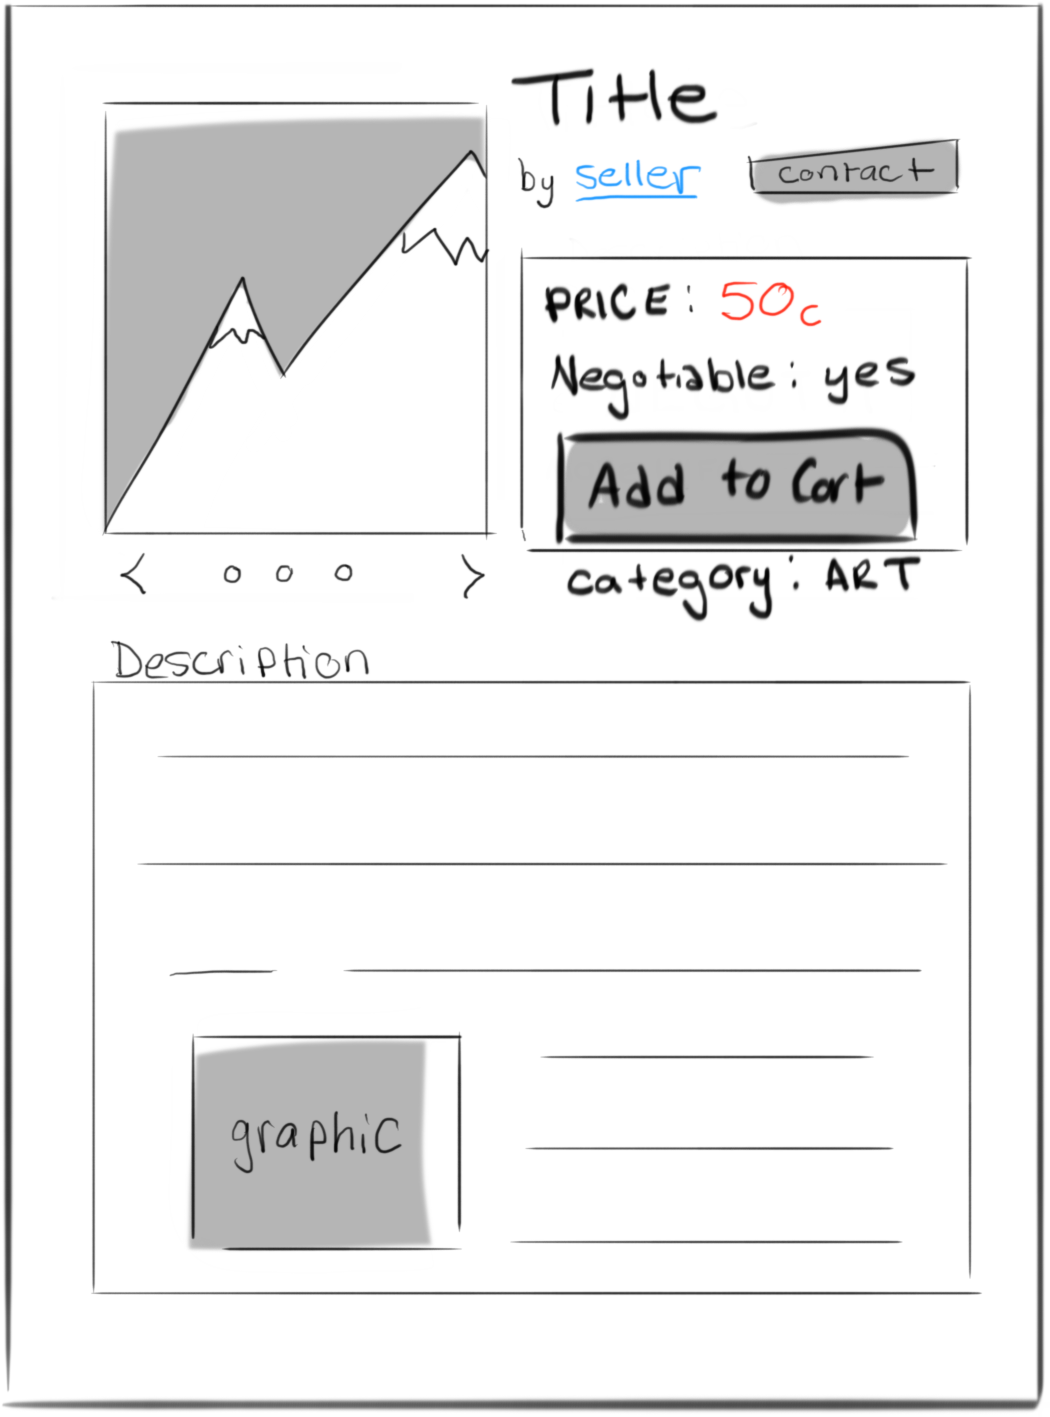
\includegraphics[width=\linewidth]{./pictures/product.png}
		  \caption{On product page, user can add item to cart then enter the cart.}
		  \label{fig:buyer3}
		\end{figure}
		
		\begin{figure}
		  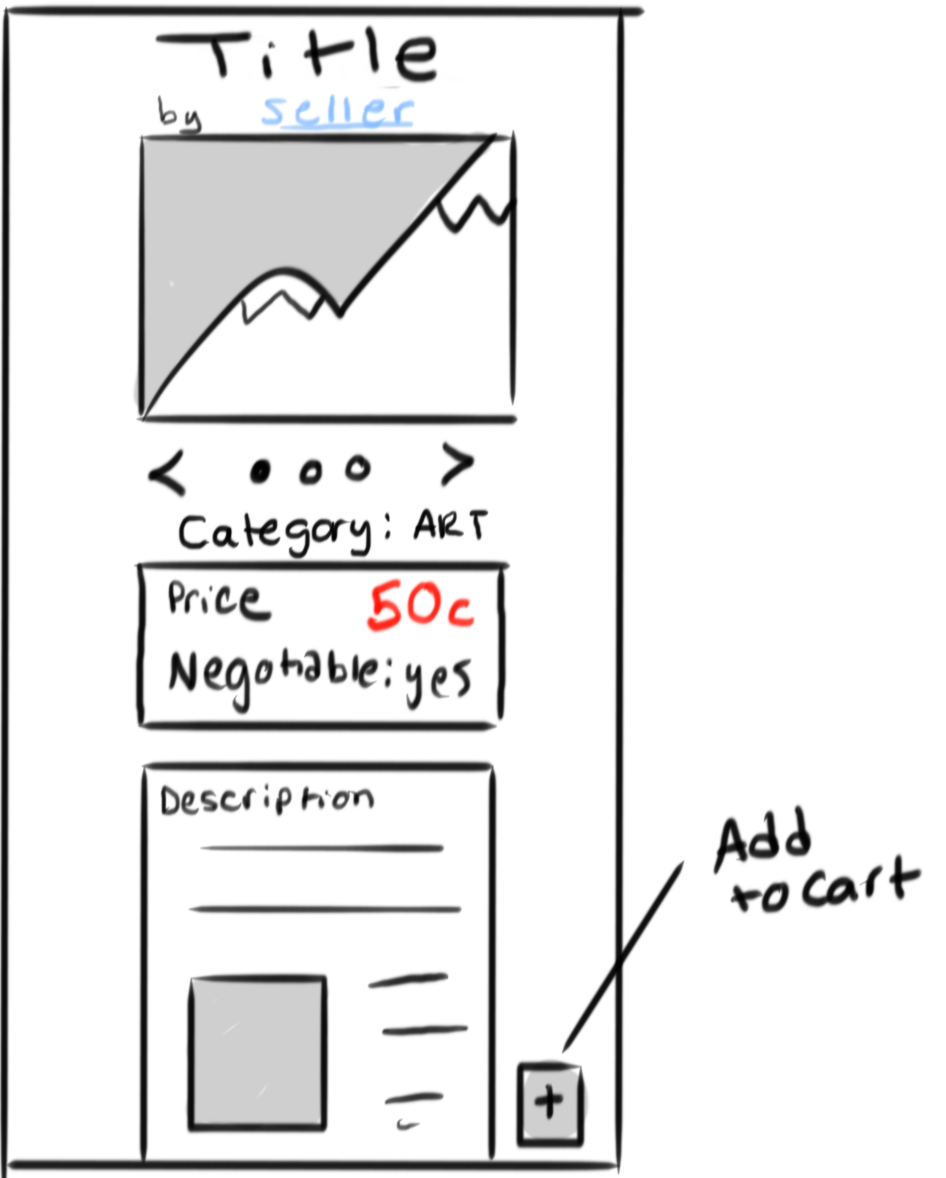
\includegraphics[width=\linewidth]{./pictures/product_mobile.png}
		  \caption{Mobile version.}
		  \label{fig:mobile8}
		\end{figure}
		
		\begin{figure}
		  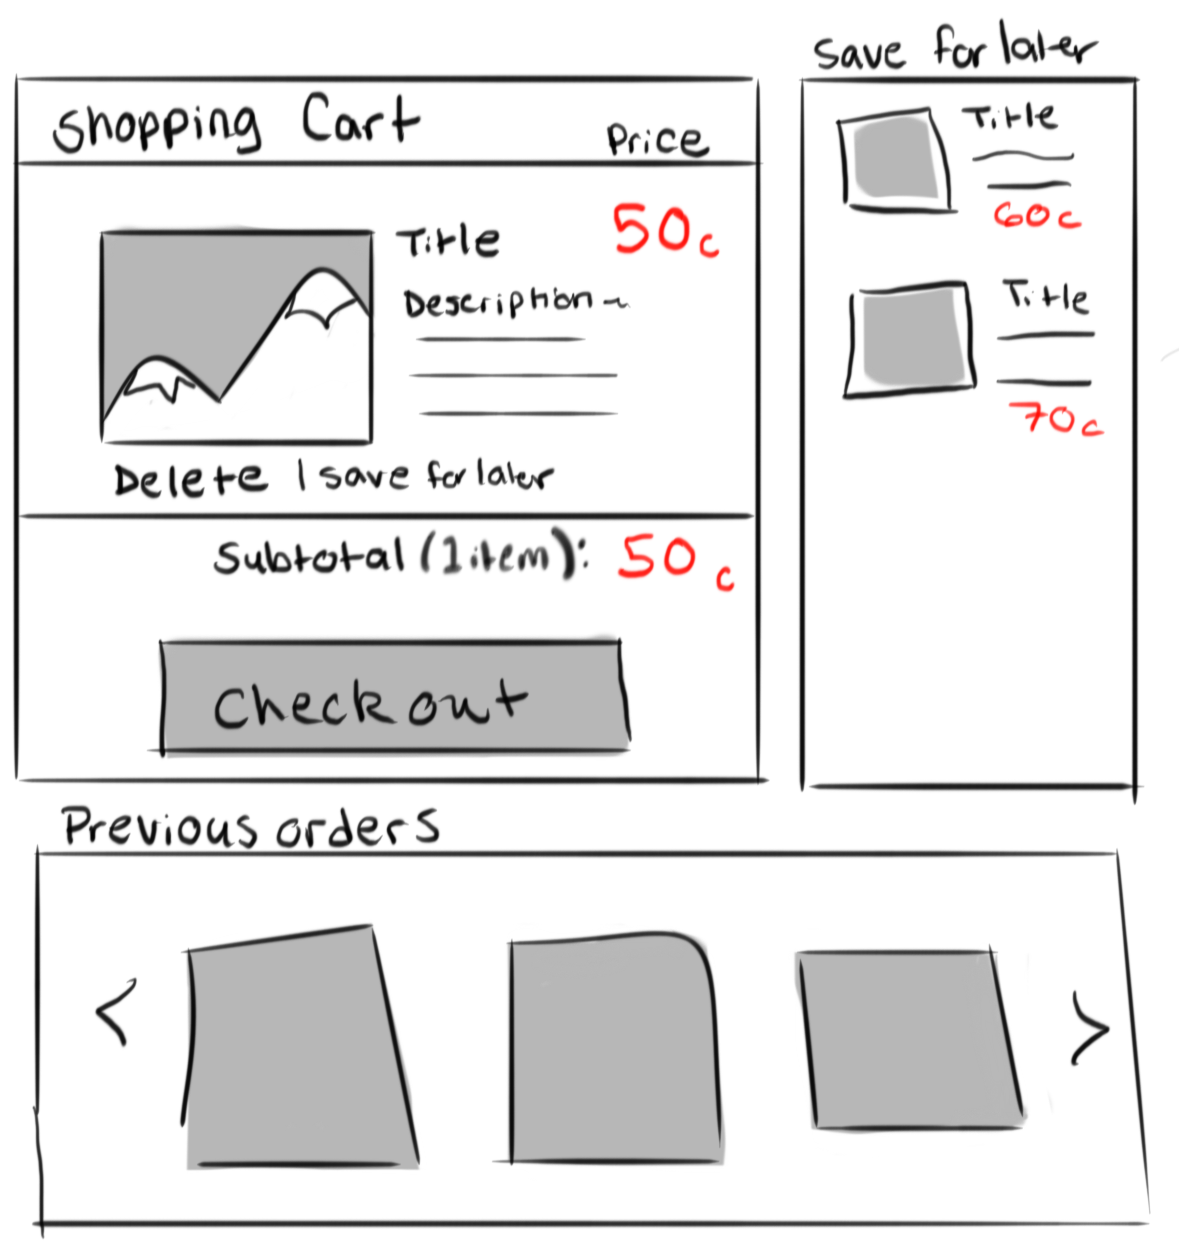
\includegraphics[width=\linewidth]{./pictures/shopping_cart.png}
		  \caption{On cart page, user can proceed to checkout.}
		  \label{fig:buyer4}
		\end{figure}
		
		\begin{figure}
		  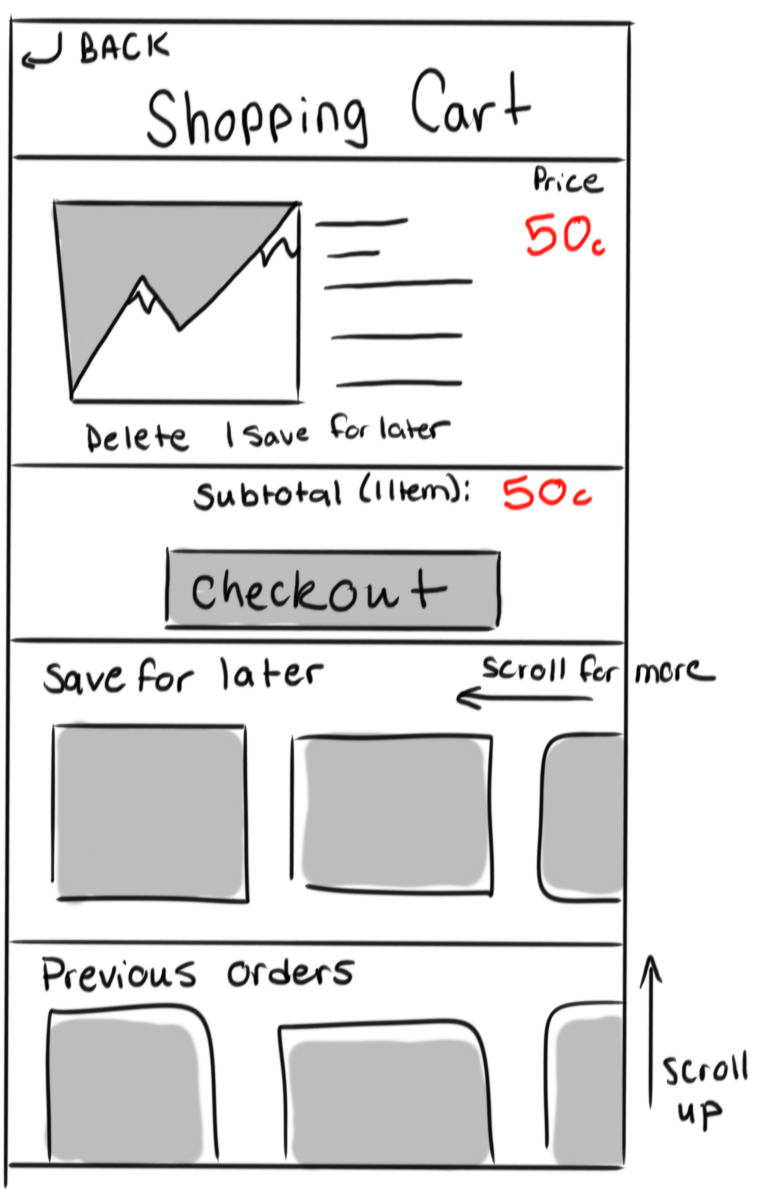
\includegraphics[width=\linewidth]{./pictures/shopping_cart_mobile.png}
		  \caption{Mobile version.}
		  \label{fig:mobile9}
		\end{figure}
		
		\begin{figure}
		  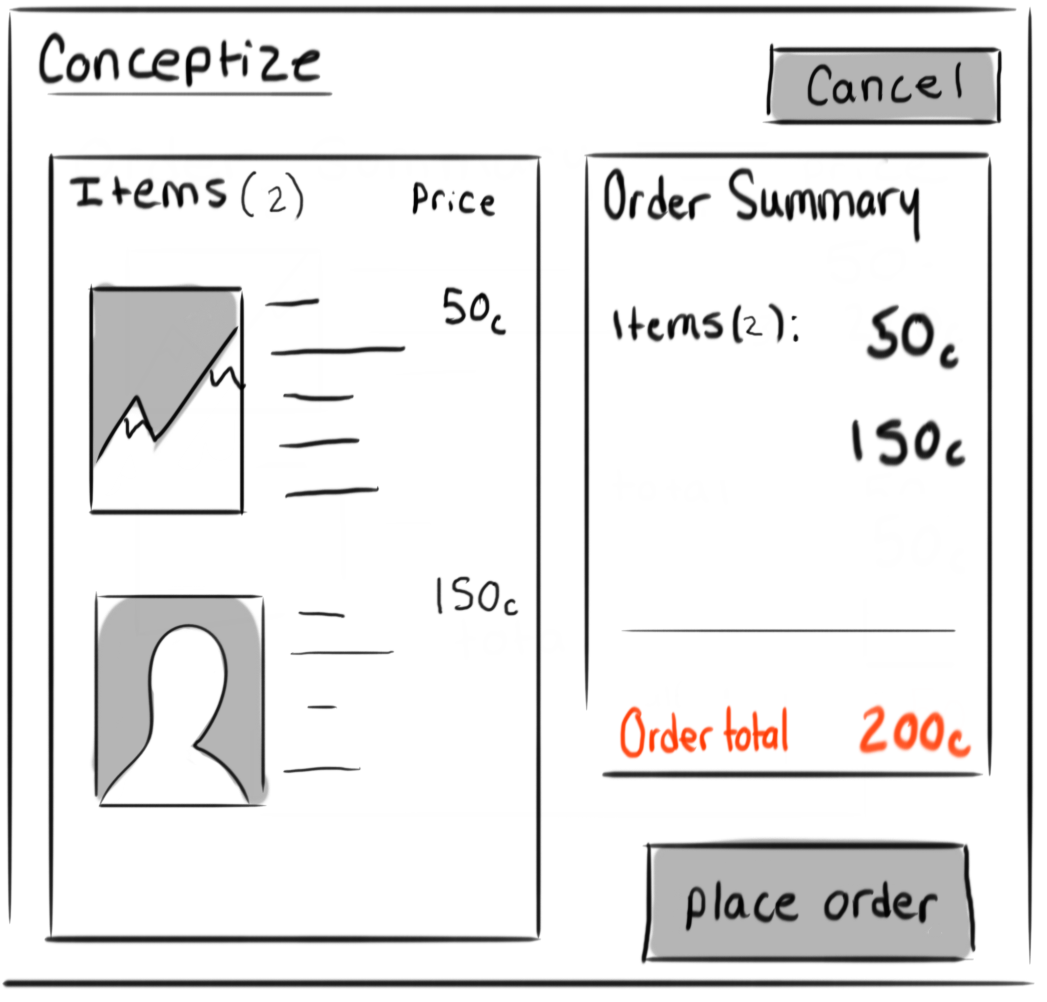
\includegraphics[width=\linewidth]{./pictures/checkout.png}
		  \caption{On checkout, user completes payment processing and places order.}
		  \label{fig:buyer5}
		\end{figure}
		
		\begin{figure}
		  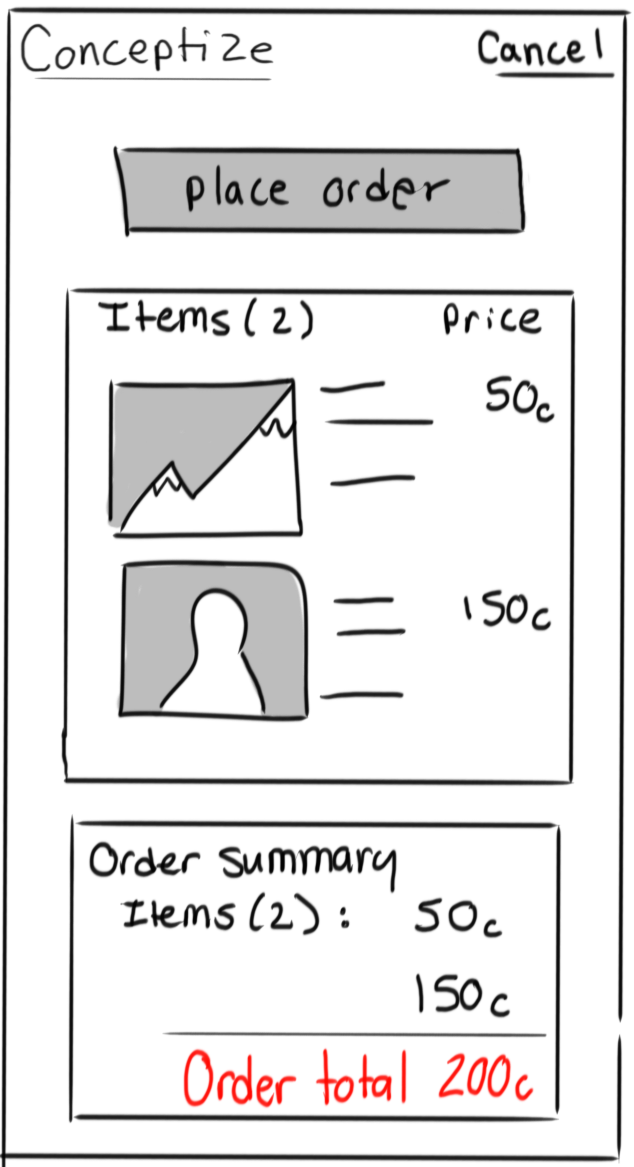
\includegraphics[width=\linewidth]{./pictures/checkout_mobile.png}
		  \caption{Mobile version.}
		  \label{fig:mobile10}
		\end{figure}
		
		\begin{figure}
		  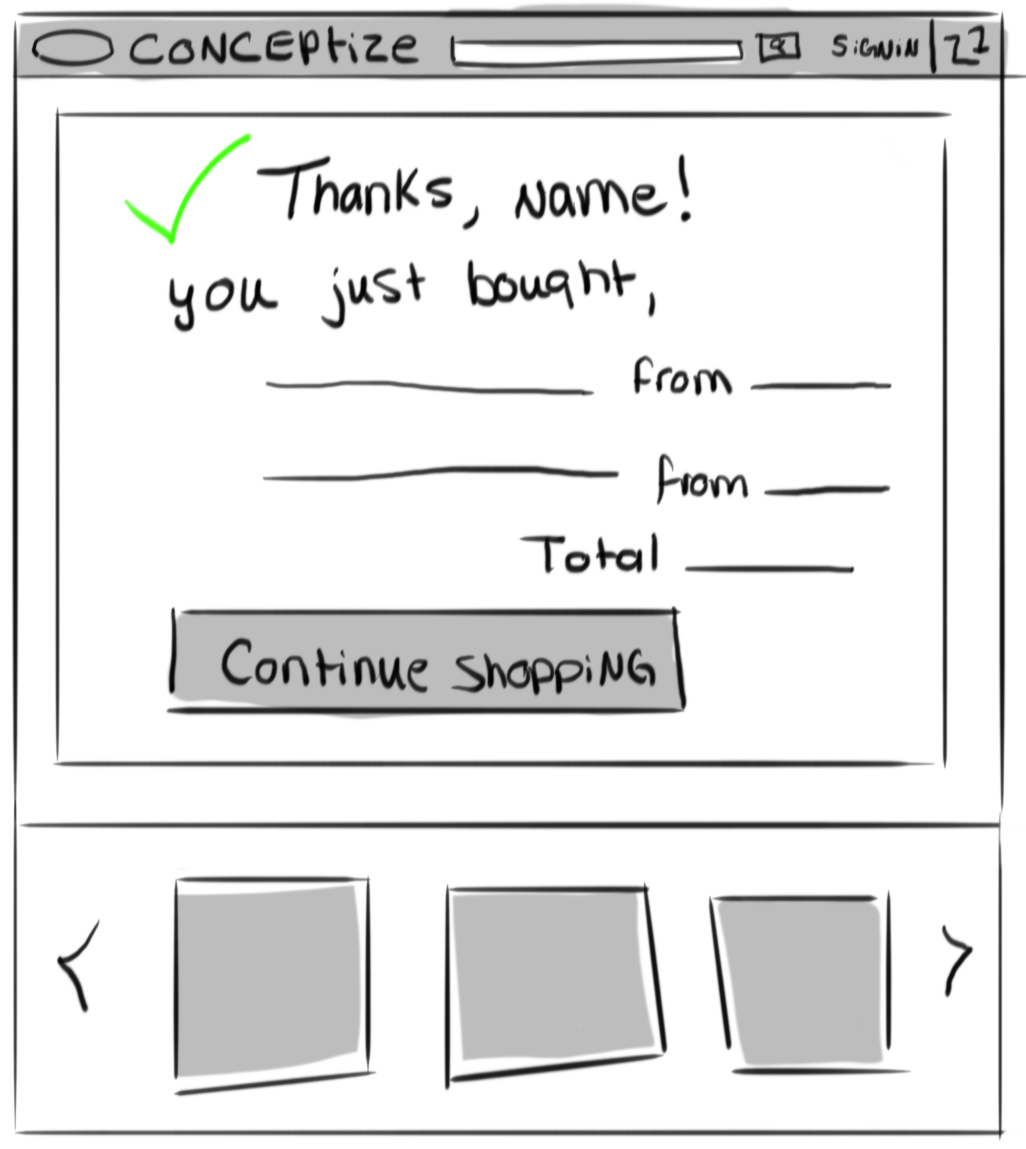
\includegraphics[width=\linewidth]{./pictures/confirmation.png}
		  \caption{The user is given confirmation that their order is now complete.}
		  \label{fig:buyer6}
		\end{figure}		
		
		\begin{figure}
		  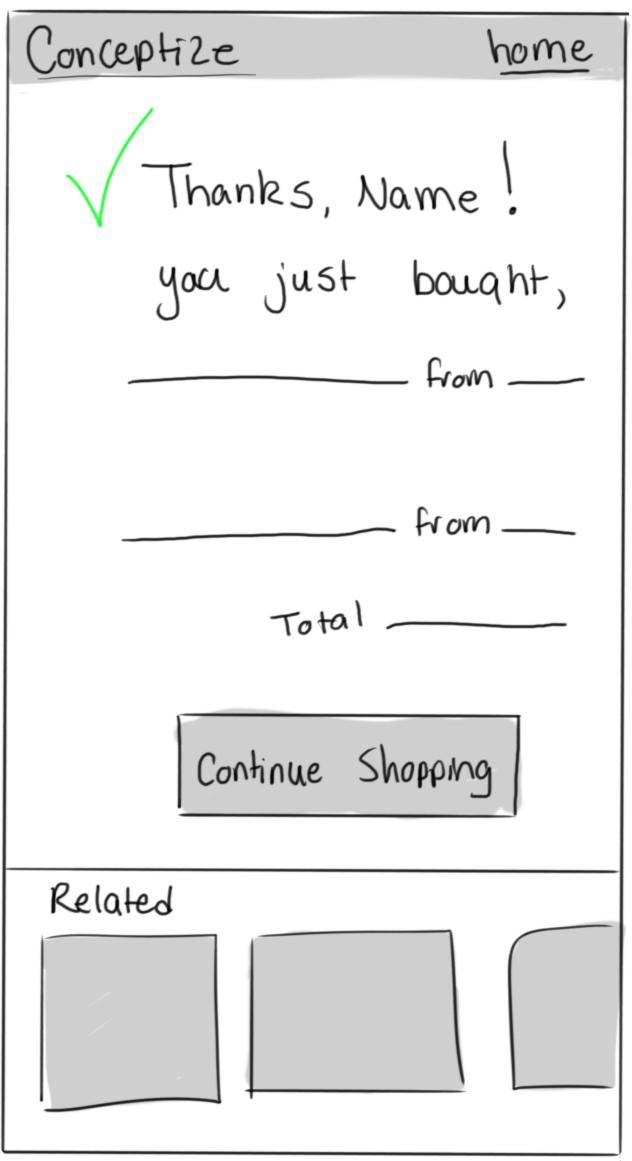
\includegraphics[width=\linewidth]{./pictures/confirmation_mobile.png}
		  \caption{Mobile version.}
		  \label{fig:mobile11}
		\end{figure}
	\end{enumerate}
	Check additional pictures in the .zip containing mobile views and additional pages
	
	\newpage
	\section{ER Diagram}
	\subsection{Prologue}
		Explain the purpose of this section here
		
	\begin{figure}[!htb] %ER Diagram here
		%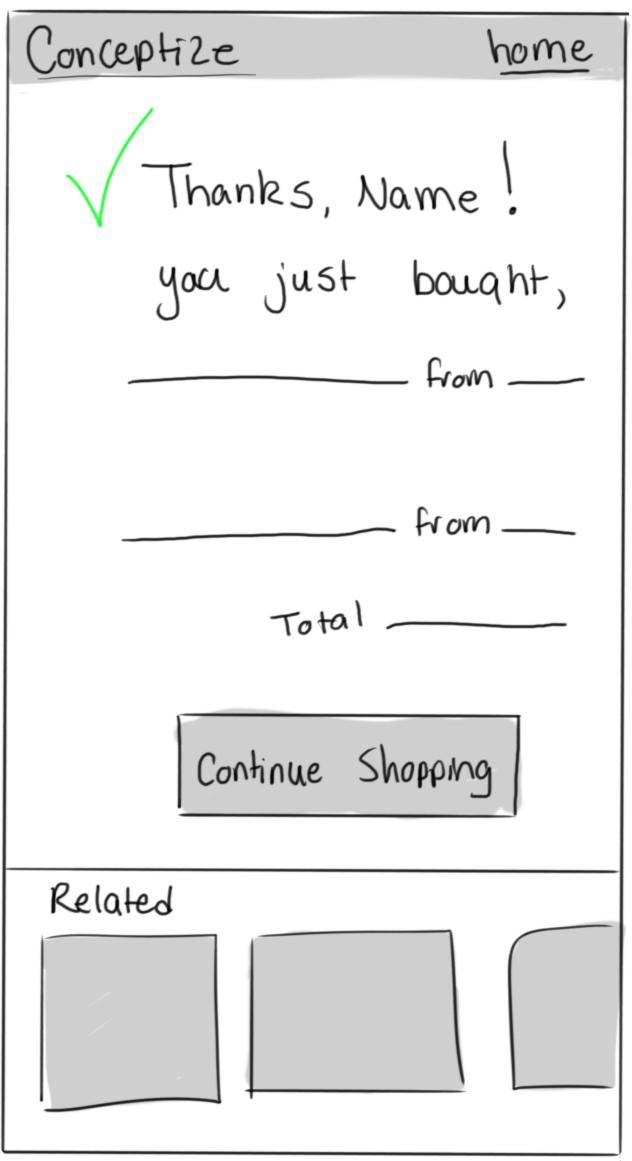
\includegraphics[width=\linewidth]{./pictures/confirmation_mobile.png}
		%\caption{ER Diagram for our website database design}
		%\label{fig:ERDiagram}
	\end{figure}

	\newpage

	\subsection{Table Design} %Tables in ER here
	
	Table 1: 
	
	\begin{table}[!htb]
		\begin{tabular}{|c|c|c|c|c|c|c|c|}
			\hline Primary Key & Field Name & Data Type & Non-null & Unique & Binary & Foreign Key & Comments \\
			\hline Search & V & V & V & V & V & V & V\\
			\hline Filter & V & V & V & V & V & V & V\\
			\hline Recommend & V & V & V & V & V & V & X\\
			\hline Pagination & V & V & X & V & V & X & V\\
			\hline Copyright & V & X & O & X & X & X & X\\
			\hline Premium currency & V & X & V & O & O & V & X\\
			\hline Auction & V & X & X & X & V & X & O\\
			\hline Security & V & V & V & V & V & V & X\\
			\hline Economy & V & X & X & X & X & X & X\\
			\hline User Profile & V & X & V & X & X & V & O\\
			\hline Private message & V & V & V & O & O & V & X\\
			\hline Forced login & V & X & V & X & O & V & X\\
			\hline Reviewed by Site & V & X & X & V & V & O & X\\
			\hline Chatrooms & V & X & V & X & X & V & O\\
			\hline Categorization & V & V & V & V & V & V & V\\
			\hline Seller Rating & V & V & X & V & V & X & X\\ 
			\hline
		\end{tabular}
		\caption{V: Able to perform the task; X: Unable to perform the task; O: Able to perform the task with poor interactive design}
		\end{table}
	
	Table 2
	\begin{table}[!htb]
		\begin{tabular}{|c|c|c|c|c|c|c|c|}
			\hline  & Our System & Fiverr & DeviantArt & Amazon & Ebay & AminoApps & Craigslist \\
			\hline Search & V & V & V & V & V & V & V\\
			\hline Filter & V & V & V & V & V & V & V\\
			\hline Recommend & V & V & V & V & V & V & X\\
			\hline Pagination & V & V & X & V & V & X & V\\
			\hline Copyright & V & X & O & X & X & X & X\\
			\hline Premium currency & V & X & V & O & O & V & X\\
			\hline Auction & V & X & X & X & V & X & O\\
			\hline Security & V & V & V & V & V & V & X\\
			\hline Economy & V & X & X & X & X & X & X\\
			\hline User Profile & V & X & V & X & X & V & O\\
			\hline Private message & V & V & V & O & O & V & X\\
			\hline Forced login & V & X & V & X & O & V & X\\
			\hline Reviewed by Site & V & X & X & V & V & O & X\\
			\hline Chatrooms & V & X & V & X & X & V & O\\
			\hline Categorization & V & V & V & V & V & V & V\\
			\hline Seller Rating & V & V & X & V & V & X & X\\ 
			\hline
		\end{tabular}
		\caption{V: Able to perform the task; X: Unable to perform the task; O: Able to perform the task with poor interactive design}
		\end{table}
	
	
	
\end{document}
